%%%%%%%%%%%%%%%%%%%%%%%%%%%%%%%%%%%%%%%%%%%%%%%%%%%%%%%%%%%%%%%%%%%%%%%%%%%%%%%%
\chapter{Постановка задачи и выбор средств реализации}
%%%%%%%%%%%%%%%%%%%%%%%%%%%%%%%%%%%%%%%%%%%%%%%%%%%%%%%%%%%%%%%%%%%%%%%%%%%%%%%%

***

%%%%%%%%%%%%%%%%%%%%%%%%%%%%%%%%%%%%%%%%%%%%%%%%%%%%%%%%%%%%%%%%%%%%%%%%%%%%%%%%
\section{Задача инструментирования}
%%%%%%%%%%%%%%%%%%%%%%%%%%%%%%%%%%%%%%%%%%%%%%%%%%%%%%%%%%%%%%%%%%%%%%%%%%%%%%%%

***

%%%%%%%%%%%%%%%%%%%%%%%%%%%%%%%%%%%%%%
\subsection{Детальная постановка задачи}
%%%%%%%%%%%%%%%%%%%%%%%%%%%%%%%%%%%%%%

=== ЧЕРНОВОЙ ВАРИАНТ ===

Необходимо разработать мультиязычную расширяемую программную систему, позволяющую производить автоматическое инструментирование исходного текста программы в соответствии с правилами, задаваемыми пользователем такой системы.

Следует принять во внимание возможность пользователя выполнять инструментирование исходных текстов синтаксически-корректной программы, созданной с использованием любого языка программирования, грамматику которого может описать пользователь формально с использованием языка TXL.

Особое внимание следует уделить возможности инструментирования основных управляющих конструкций выбранного пользователем языка программирования.

=== ЧЕРНОВОЙ ВАРИАНТ ===

***

***
Ключевыми идеями системы являются:
\begin{itemize}[noitemsep]
  \item Оперирование контекстами инструментирования как некоторыми множествами.
  \item Использование одного прохода по дереву разбора для осуществления требуемых манипуляций (вставки фрагментов программного кода).
\end{itemize}

***

%%%%%%%%%%%%%%%%%%%%%%%%%%%%%%%%%%%%%%
\subsection{Обработка деревьев разбора}
%%%%%%%%%%%%%%%%%%%%%%%%%%%%%%%%%%%%%%

***

Способы обхода древовидных структур данных:
* обход вглубину
* обход вширину

Исходя из функциональной природы языка TXL, *

***

Приведенные выше рассуждения приводят к формулировке метода, который способен решить поставленную задачу.

***

%%%%%%%%%%%%%%%%%
\subsubsection{Нисходящий однопроходный метод}
%%%%%%%%%%%%%%%%%

Основная идея -- спуск по дереву разбора (CST) от корневого узла к листьям, собирая по пути следования информацию для определения контекста, в котором находятся обрабатываемые/инструментируемые узлы.
\nomenclature{CST}{Concrete Syntax Tree -- конкретное дерево разбора}

Обход "в глубину" (DFT).
\nomenclature{DFT}{Depth-First Traversal -- метод обхода графовой структуры, состоящий в том, чтобы идти ``вглубь'' графа, насколько это возможно}

***

Основная идея нисходящего подхода заключается в постепенном спуске по дереву разбора, которое генерирует внутри себя утилита TXL, от корневого узла к листьям, сохраняя по пути следования информацию для определения контекста, в котором находятся обрабатываемые узлы и выполняется инструментирование.

Данный метод хорошо соотносится с функциональной природой языка TXL, с помощью которого можно описать цепочку вызовов взаимосвязанных функций для обработки различных вложенных типов узлов дерева разбора.

Однако, данный метод подходит только для таких языков программирования, которые соответствуют принципу вложенности синтаксических элементов, т.е. программы, составленные на данных языках программирования соответствуют \textit{структурной парадигме} программирования [***].

***

%%%%%%%%%%%%%%%%%
\subsubsection{Нисходящий многопроходный метод}
%%%%%%%%%%%%%%%%%

***

%%%%%%%%%%%%%%%%%%%%%%%%%%%%%%%%%%%%%%
\subsection{Контексты инструментирования}
%%%%%%%%%%%%%%%%%%%%%%%%%%%%%%%%%%%%%%

иснтрументирование подразумевает использование некоторых контекстов, поэтому с ними было бы удобно работать как с множествами

Проблема представления деревьев в виде множеств
Или сопоставления деревьев и множеств
правила грамматики могут описывать бесконечные деревья

\begin{figure}[H]
	\centering
	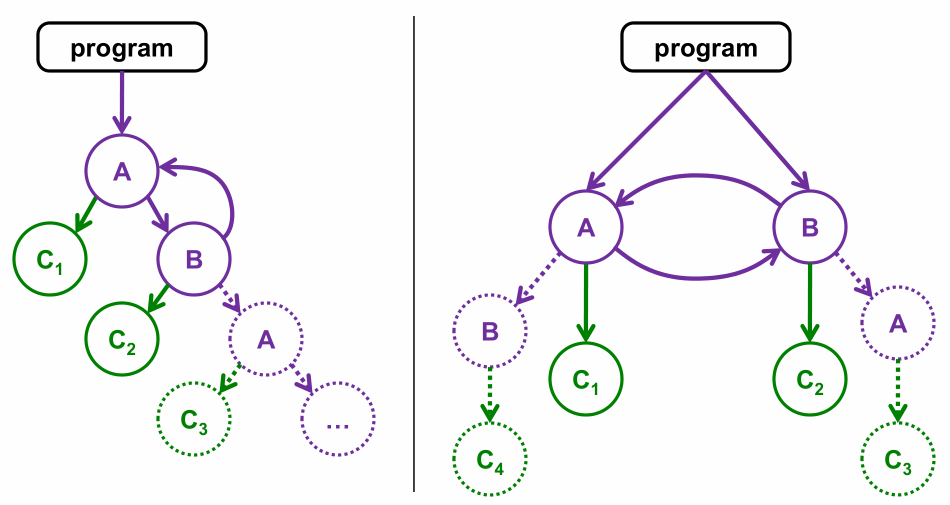
\includegraphics[width=3.2in]{tree_inf}
	\caption{Пример дерева разбора с повторением типов узлов}
	\label{fig:tree_inf}
\end{figure}

рассмотрим пример: пусть $A$, $B$, $C$, $D$ -- ***

какие есть способы описания ограничений в TXL
один из них -- КНФ

исходя из этого
$A * B + C * D$
переходит в
$(A + C) * (A + D) * (B + C) * (B + D)$

***

Поскольку язык, который используется для программирования утилиты TXL, принадлежит к семейству функциональных языков программирования, это ограничение заставляет передавать собираемую информацию посредством аргументов/параметров, с которыми вызываются последующие функции в цепочке.

***

теперь необходимо распределить эти ограничения по функциям в соответствии с узлами из дерева рабора, которые содержат значения, которые нужно проверить

***

\begin{figure}[H]
	\centering
	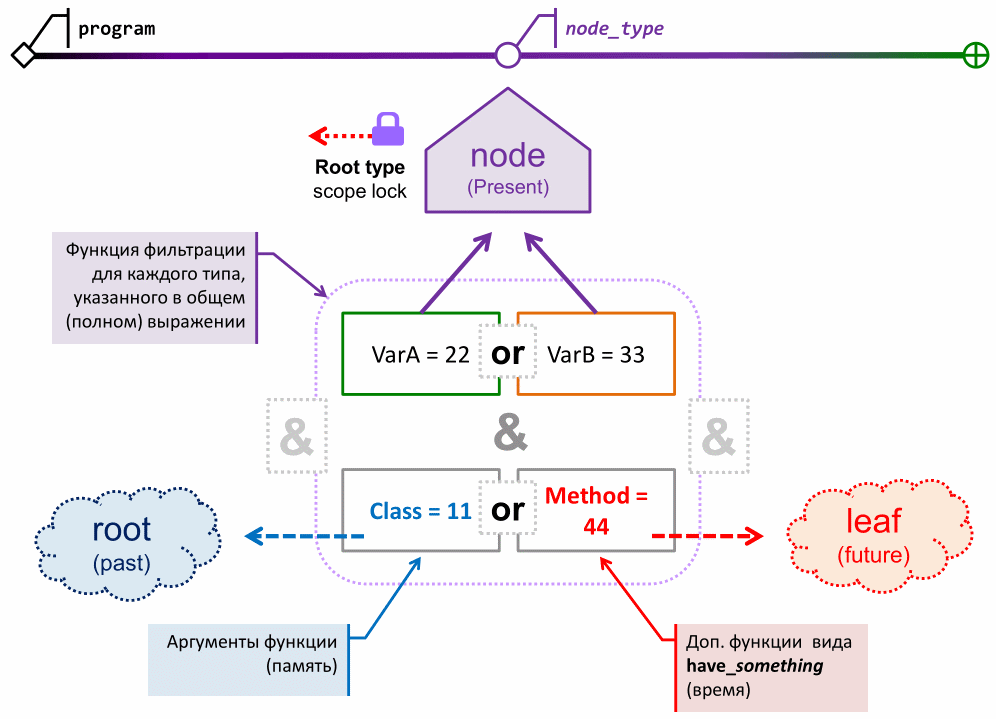
\includegraphics[width=3.5in]{filter_abstract}
	\caption{Обобщенная модель функции фильтрации по контексту инструментирования.}
	\label{fig:filter_abstract}
\end{figure}

***

Группировка по типам узлов дерева разбора, которые содержат данные, на основе которых выполняется принятие решения о принадлежности к контексту инструментирования. Иными словами -- содержат значения, проверяемые ограничениями из формул.

\begin{figure}[H]
	\centering
	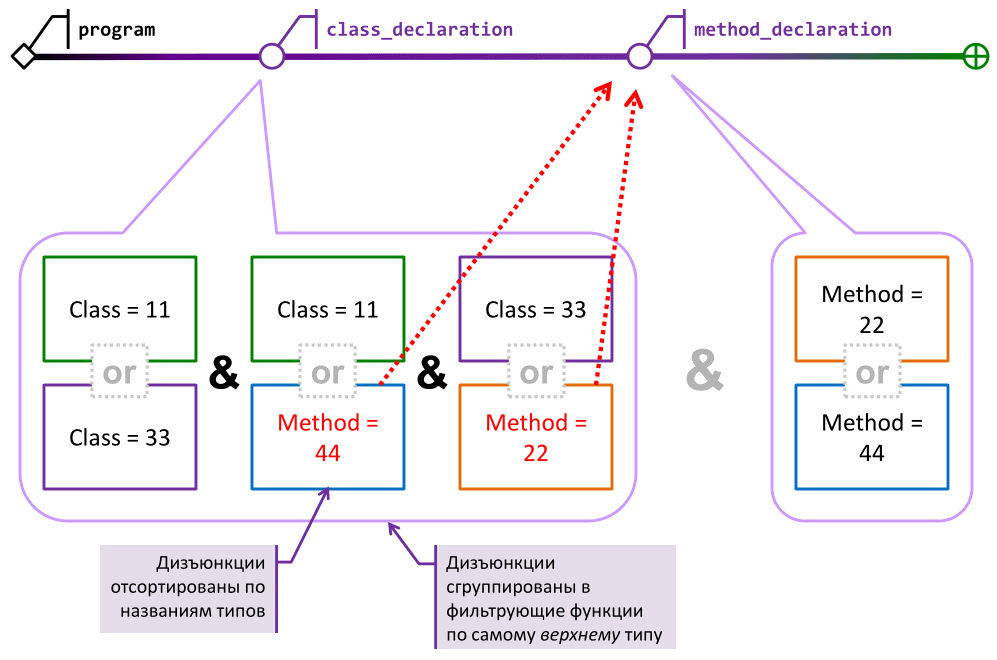
\includegraphics[width=3.2in]{filter_types}
	\caption{Группировка ограничений. По типам узлов.}
	\label{fig:filter_types}
\end{figure}

***

Группировка с применением дополнительных функций сбора информации.

\begin{figure}[H]
	\centering
	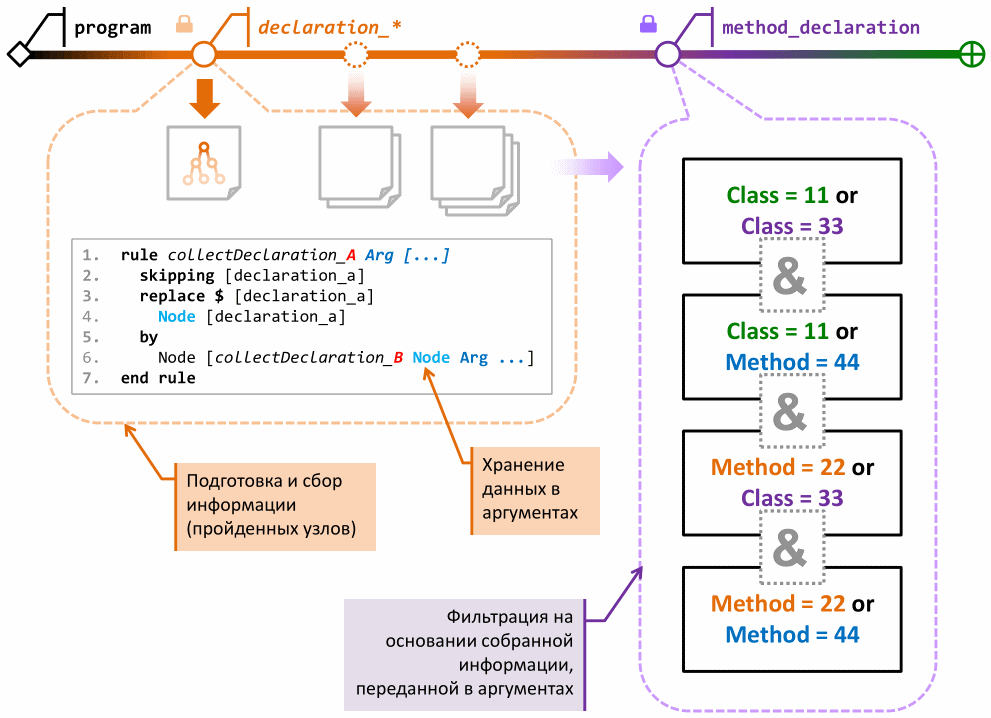
\includegraphics[width=3.7in]{filter_collect}
	\caption{Группировка ограничений. Дополнительные функции.}
	\label{fig:filter_collect}
\end{figure}

***

%%%%%%%%%%%%%%%%%%%%%%%%%%%%%%%%%%%%%%%%%%%%%%%%%%%%%%%%%%%%%%%%%%%%%%%%%%%%%%%%
\section{??? Выбор пути (глобально)}
%%%%%%%%%%%%%%%%%%%%%%%%%%%%%%%%%%%%%%%%%%%%%%%%%%%%%%%%%%%%%%%%%%%%%%%%%%%%%%%%

***

Инструментирование исходного текста.
Только добавление текста -- вцелом порядок может быть такой: удаление, обновление, добавление.
Правила инструментирования задаются декларативно.
Зависимые правила?

***

%%%%%%%%%%%%%%%%%%%%%%%%%%%%%%%%%%%%%%%%%%%%%%%%%%%%%%%%%%%%%%%%%%%%%%%%%%%%%%%%
\section{Средства разработки}
%%%%%%%%%%%%%%%%%%%%%%%%%%%%%%%%%%%%%%%%%%%%%%%%%%%%%%%%%%%%%%%%%%%%%%%%%%%%%%%%

***
TXL, C++, Boost library, argparse, tinyxml2

%%%%%%%%%%%%%%%%%%%
\subsection{Выполнение трансформаций текста программ}
%%%%%%%%%%%%%%%%%%%

***
про TXL

Для осуществления трансформаций исходных текстов программ, созданных с помощью большого разнообразия различных языков рограммирования, необходимо либо реализовать собственное средство, позволяющее выполнять требуемые преобразования с учетом нюансов отдельно взятых языков программирования, либо использовать существующее средство или язык такие как, например, ASF+SDF, Stratego/XT, Refal, TXL или подобные им.

\nomenclature{ASF}{Algebraic Specification Formalism}
\nomenclature{SDF}{Syntax Definition Formalism}

[http://txl.ca/txl-abouttxl.html]
TXL -- это язык программирования, специально разработанный для поддержки задач анализа компьютерного программного обеспечения и преобразования исходных текстов посредством структурной трансформации на основе правил как парадигмы быстрого решения сложных вычислительных задач.
Язык сочетает в себе элементы функциональных и основанных на правилах языках программирования с унификацией, базирующейся на итеррационном подходе с рекурсивным сопоставлением шаблонов.

***

[http://txl.ca/txl-download.html]
FreeTxl -- это бесплатный компилятор/интерпретатор программ для языка TXL, основанный на применении XML, распространяемый лабораторией университета Куинс в Кингстоне~\ref{txl-freetxl}.

***

%%%%%%%%%%%%%%%%%%%%%%%%%%%%%%%%%%%%%%%%%%%%%%%%%%%%%%%%%%%%%%%%%%%%%%%%%%%%%%%%
\section{Выводы}
%%%%%%%%%%%%%%%%%%%%%%%%%%%%%%%%%%%%%%%%%%%%%%%%%%%%%%%%%%%%%%%%%%%%%%%%%%%%%%%%

***
